\documentclass{nime-alternate} 
\usepackage{anonymize} 		    % publish
% \usepackage[blind]{anonymize}       % blind review
\usepackage[utf8]{inputenc}
\usepackage{listings}
\usepackage{xcolor}
\begin{document}

%New colors defined below
\definecolor{codegreen}{rgb}{0,0.6,0}
\definecolor{codegray}{rgb}{0.15,0.15,0.15}
\definecolor{codepurple}{rgb}{0.58,0,0.82}
\definecolor{backcolour}{rgb}{0.95,0.95,0.92}

%Code listing style named "mystyle"
\lstdefinestyle{mystyle}{
  backgroundcolor=\color{backcolour},   commentstyle=\color{codegreen},
  keywordstyle=\color{magenta},
  numberstyle=\tiny\color{codegray},
  stringstyle=\color{codepurple},
  basicstyle=\ttfamily\footnotesize,
  breakatwhitespace=false,         
  breaklines=true,                 https://www.overleaf.com/project/603c50f96f2e08e673a4587b
  captionpos=b,                    
  keepspaces=true,                 
  numbers=left,                    
  numbersep=5pt,                  
  showspaces=false,                
  showstringspaces=false,
  showtabs=false,                  
  tabsize=2
}

%"mystyle" code listing set
\lstset{style=mystyle}

% \conferenceinfo{}

\title{DreamSound: Deep Activation Layer Sonification}

\label{key}
\numberofauthors{2}
\author{
\alignauthor
\anonymize{Federico Camara Halac}\\
       \affaddr{\anonymize{Ohio State University}}\\
       \affaddr{\anonymize{School of Music --- ACCAD}}\\
       \affaddr{\anonymize{1813 North High Street}}\\
       \affaddr{\anonymize{Columbus, Ohio}}\\
       \email{\anonymize{camarahalac.1@osu.edu}}
\alignauthor
\anonymize{Matias Delgadino}\\
       \affaddr{\anonymize{Oxford University}}\\
       \affaddr{\anonymize{Mathematical Institute}}\\
       \affaddr{\anonymize{Andrew Wiles Building, Woodstock Road}}\\
       \affaddr{\anonymize{Oxford, OX2 6GG}}\\
       \email{\anonymize{matias.delgadino@maths.ox.ac.uk}}
}

\date{24 January 2021}
\maketitle
\begin{abstract}
Deep Learning in raw audio-based musical contexts is yet a largely unexplored field. In other artistic contexts, such as the visual arts, Deep Learning models have been not only used for classification, but also for image generation. In this paper, we present an adaptation of the Deep Dream project into an audio-based musical context. Using raw audio and sonic feedback at every stage, we created a rapid prototype by sonifying a network's activation layers. Our results show the most interesting results when recursively applying an FFT filter built from the gradients obtained from an input soundfile and its loss. 

\end{abstract}

\keywords{Machine Learning, Sonification, Classification, Deep Dream}
% \ccsdesc[500]{Applied computing~Sound and music computing}
% \ccsdesc[300]{Applied computing~Performing arts}
% \ccsdesc[300]{Human-centered computing~Activity centered design}
% \ccsdesc[100]{Information systems~Music retrieval}

% \printccsdesc
\section{Introduction}
Deep Learning in raw audio-based musical contexts is yet a largely unexplored field. On one hand, Deep Learning has been only recently taken in by the Music Information Retrieval community, mostly for unsuperivsed classification and Computational Musicology analysis. On the other, much of the Deep Learning audio-related work so far relates to speech-related tasks like recognition or generation. Therefore, while there is an ever growing interest in applying Machine Learning techniques to music, there is little work at the intersection of Deep Learning and audio-based musical tasks. 

One recent example at this intersection is WaveNet and WaveGan. These two projects are raw-audio based, the former aimed towards speech generation, the latter to more general sound generation. These architectures are both aimed to generate short-length audio files using some variation of the Generative Adversarial Network architecture. Another example is Kwgan, an extension of the WaveGan architecture aimed to build large-scale audio databases for electroacoustic music material. In this case, raw audio is inputted for training and outputted for artistic or musically relevant contexts.

In other artistic contexts, such as the visual arts, Deep Learning models have been not only used for classification, but also for image generation. This is the case of the Deep Dream project, geared towards image generation using layer information within a Deep Learning, InceptionNet, architecture previously built and trained for classification. The output of the Deep Dream is an image that is either modified or completely generated by the neural network itself, hence calling it 'dream'.

In the present paper, we present DreamSound,\footnote{\url{https://github.com/fdch/dreamsound}} an adaptation of the Deep Dream project into an audio-based musical context. DreamSound uses YAMNet, a sound classification deep convolutional network, so as to obtain relevant layer information for raw audio generation. 

In section 1 we present our approach and the limitations we have found. In section 2, we expose our methods and technques. In section 3, we present our results and briefly discuss them in context.

\section{Approach}
Our project begins as a rapid prototype for DeepSounds by sonifying a convolutional neural network's activation layers. We carried out our remote and collaborative work within the Google Collab environment using Python, namely with tensorflow, numpy, and librosa. While there are many available trained models for sound classification, we have chosen a general sound source classifier YAMNet \footnote{\url{https://github.com/tensorflow/models/tree/master/research/audioset/yamnet}}. YAMNet is a pretrained Deep Neural Network classifier using the Mobilenet depthwise-separable convolution architecture, \footnote{\url{https://arxiv.org/abs/1704.04861}} with a final activation layer containing most relevant features for classification. On one hand, YAMNet enables a quick prototyping of the DreamSound generator, since it is built and distributed as a tensorflow model within a git repository. On the other, the relatively simple architecture of this network sheds clarity in the process of sound dreaming using neural networks. To this end, our goal is to share our process and preliminary results with the computer music community so as to make deep learning structures easier to grasp. Therefore, two important aspects need to be mentioned. The first is the generality of audio sources within the chosen dataset. 
\begin{figure*}[htbp]
       \centering
              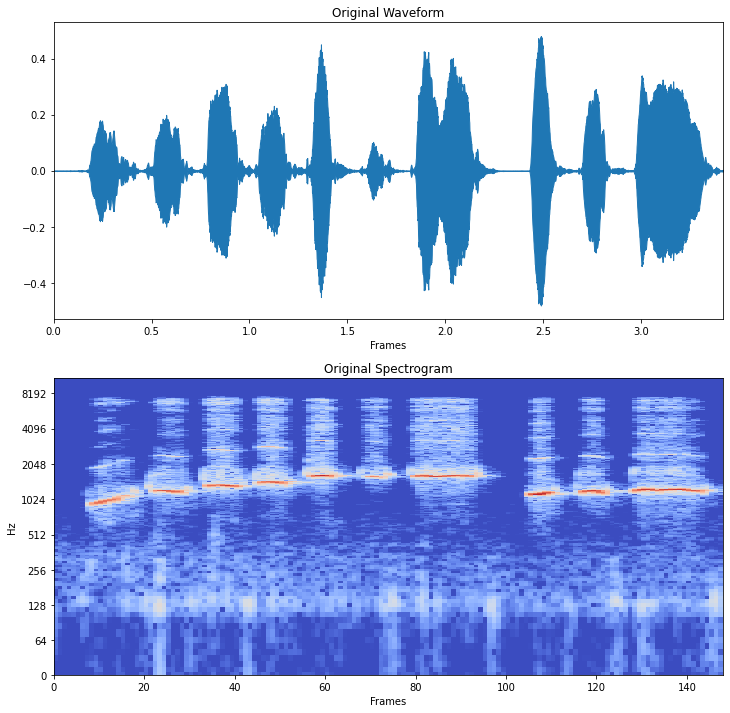
\includegraphics[width=0.5\textwidth]{dreamsound/original-waveform.png}
       \caption{Original Sound File: Whisteling}
       \label{fig:img-0}
\end{figure*}
YAMNet has been previously trained with 521 audio classes based on the AudioSet-YouTube \footnote{\url{https://research.google.com/audioset}} corpus. Since our prototype is meant for fast showcasing of the main DreamSound idea, this general raw audio database with short, mostly non-musical fragments. Therefore, we sacrificed any application of this system with other contextually/musically relevant sonic scenarios to favor a quick presentation of the idea. The second aspect relates to machine learning sonification. While most machine learning models have a way to visually represent data in graphs, there is very little research into the sonification of this data. Given that our prototipe uses sound as output, our approach is a sonification approach which takes advantage on listening to changes in the audio so as to grasp how a deep activation layer identifies sounds for classification. In fact, we have worked this prototype out with continuous sonic feedback throughout.

\begin{figure*}[htbp]
       \centering
              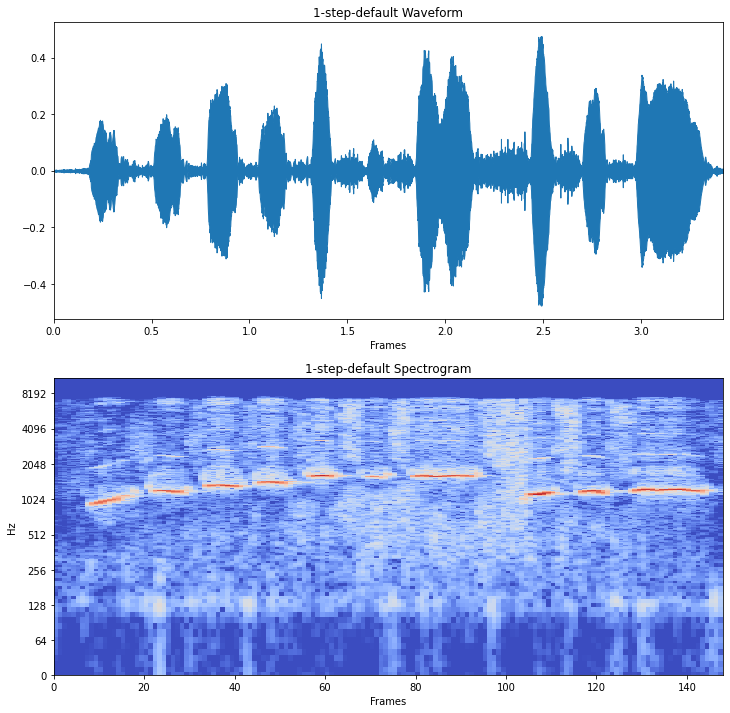
\includegraphics[width=0.5\textwidth]{dreamsound/1-step-default.png}
       \caption{One Step with default gradient addition}
       \label{fig:img-1}
\end{figure*}
\section{Method}
We based our method on the Deep Dream tutorial published by tensorflow, \footnote{\url{https://www.tensorflow.org/tutorials/generative/deepdream}} in which they implement Alexander Mordvintsev's original Deep Dream idea.\footnote{\url{https://ai.googleblog.com/2015/06/inceptionism-going-deeper-into-neural.html}} In general terms, the structure of the deep dream process involves inputting an image for classification,  grabbing the features obtained of one activation layer during that classification (aka. gradients), and combining the original image with the gradients in some way. In the tensorflow implementation, the gradients are added to the original image in small, gradual increments during a recursive process involving several passes. In our implementation, however, we had to introduce some modifications. Since we are dealing with audio, the 2-dimensional shapes of images had to be brought to one-dimensional sound arrays. Moreover, the combination of the original and the gradients is presented in different ways.
\begin{figure*}[htbp]
       \centering
              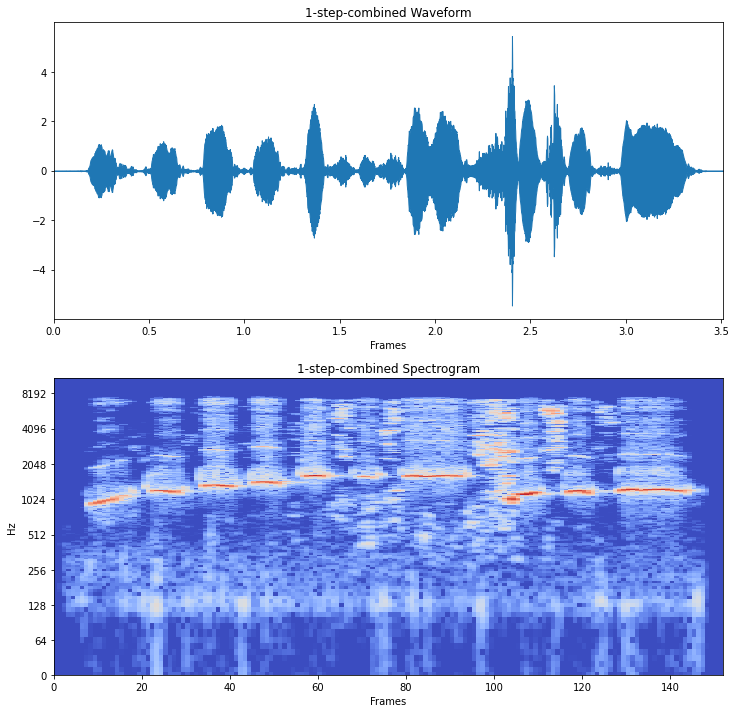
\includegraphics[width=0.5\textwidth]{dreamsound/1-step-combined.png}
       \caption{One step with original filtered with gradients}
       \label{fig:img-2}
\end{figure*}
\subsection{Algorithm Overview}
First, we pass a sound file through the model to obtain the activations with respect to one layer and get the loss across all audio frames. Then, we maximize the loss from these activations using gradient ascent with respect to the original sound file. Finally, we combine the gradients with the original sound to output a new, 'dreamed' sound.


\begin{figure*}[htbp]
       \centering
              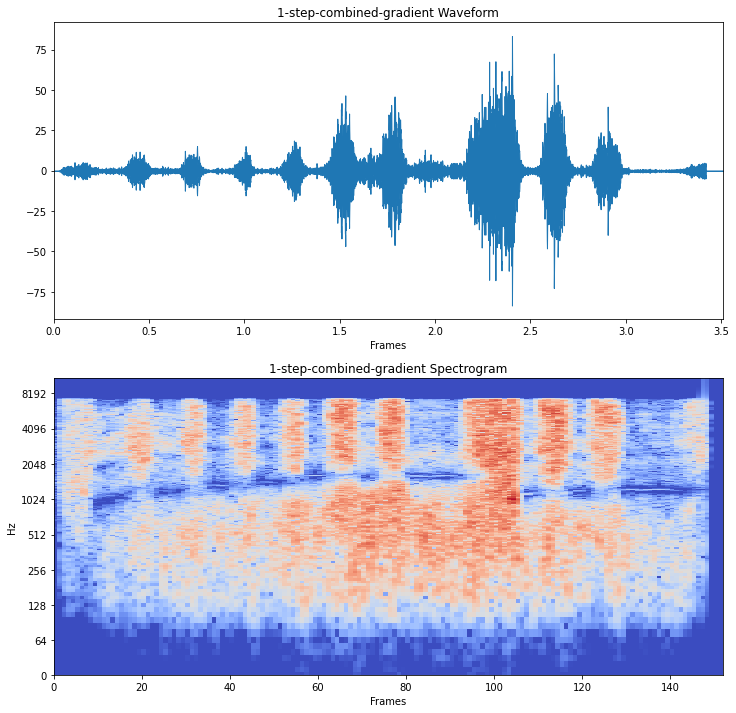
\includegraphics[width=0.5\textwidth]{dreamsound/1-step-combined-gradients.png}
       \caption{One step with gradients filtered with original}
       \label{fig:img-3}
\end{figure*}



\subsection{Calculate Loss}
We pass a sound file (See Figure \ref{fig:img-0}) through the model to obtain its activations (or scores) with respect to one layer (aka, the dream layer). Then, we take the mean accross all frames of the returned activations and return the maximum value which points to one specific class. In other words, we get the class that most represents the sound file so as to find the sum of all of its activations, thus representing the loss of the model with respect to the input.



\subsection{Gradient Ascent}
With the loss, we calcualte its gradient with respect to the input sound file, and maximize the loss so as to excite the features that most represent the input sound file within the network. In this sense, we are motivating the model to resurface what it's learnt. 


\subsection{Recursion}
Once we have the gradients, we can add them or combine them spectrally with the input sound file and listen to the output (See Figures \ref{fig:img-1}, \ref{fig:img-2} and \ref{fig:img-3}). However, if we iterate and recurse, we create a feedback loop that further excites the sonic output and we can define the number of steps and the step size of the recursion (See Figures \ref{fig:img-4}, \ref{fig:img-5}). In other words, we treat this as an feedback delay network effect with amount and amplitude values. Furthermore, we can take multiple layers simultaneously for the dream layers and see how affects the output (See Figures \ref{fig:img-6}, \ref{fig:img-7}).

\begin{figure*}[htbp]
       \centering
              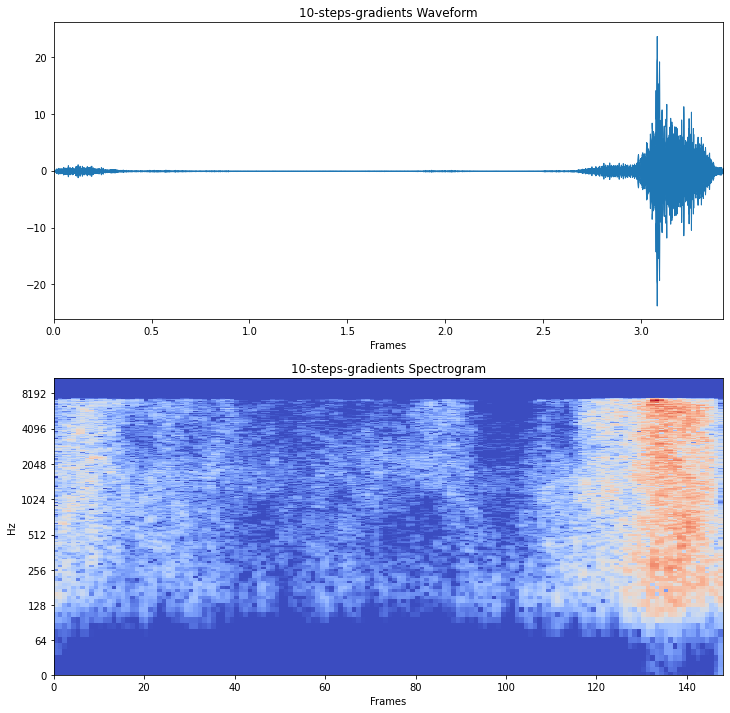
\includegraphics[width=0.5\textwidth]{dreamsound/10-steps-gradients.png}
       \caption{Recursively passing the gradients for 10 steps.}
       \label{fig:img-4}
\end{figure*}

\section{Results}
We have obtained several dreamed sound files with different parameter settings as can be seen on the presented figures across this paper.\footnote{The audio files can be listened to here: \url{https://github.com/fdch/dreamsound}} From these returned sounds, we can assess the validity of dreamsound as a deep dream implementation. In figures \ref{fig:img-1}, \ref{fig:img-2}, and \ref{fig:img-3}, we see the result of one step dream process, with different kinds of combinations between the gradients and the orignal sound. In the first example, we modify the sound usign the same method as in the deep dream tensorflow implementation. 

\begin{figure*}[htbp]
       \centering
              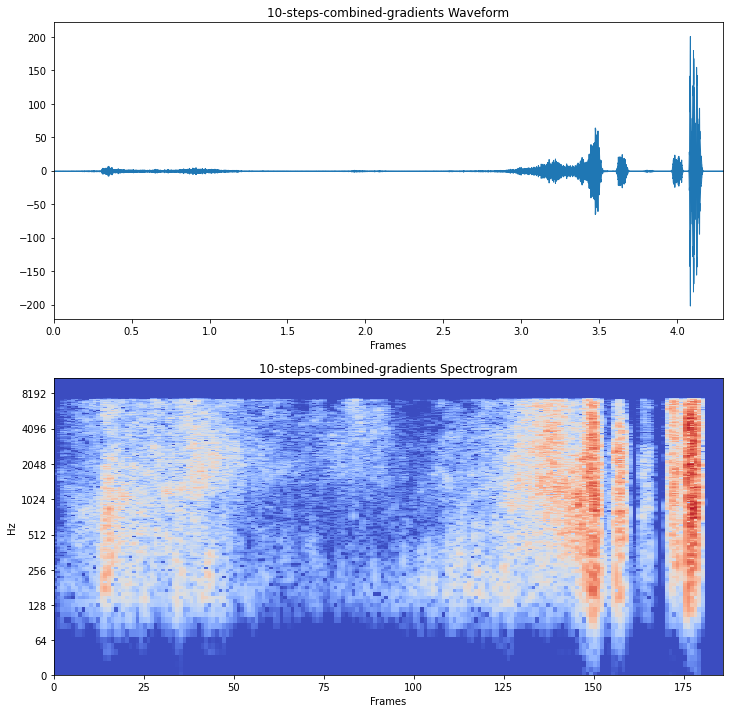
\includegraphics[width=0.5\textwidth]{dreamsound/10-steps-combined-gradients.png}
       \caption{Recursively passing the combined spectra of waveform and gradients (flipped) for 10 steps.}
       \label{fig:img-5}
\end{figure*}

This means that the gradients are added at some reduced value to the original sound file. From the result, we can listen to a slightly noisier signal. In comparison to the original sound, the noise within this new sound is enhanced when the original sound seems to fall back to silence, and it increments slightly in amplitude towards the middle section of the sound file's lenght. What we listen to here is the activations as they are represented sonically across all audio frames, so that louder portions represent the sections of the file where the most activations exists. This can be more accurately seen in Figure \ref{fig:img-3}, where we obtain the result of only sonifying the activations. However, in Figure \ref{fig:img-2}, we filter the original sound with the activations. This results in a much more insteresting sonic manipulation and result. The activations, since they evolve throghout the soundfile, create a dynamic filter concentrating towards the center of the file, which is when it resonates the most with the original sound file. This means that when we listen to the resonance, the network has the most accurate activations excited. For this step, we implemented a basic FFT filter withi tensorflow:

\begin{lstlisting}[language=Python][caption=A Custom FFT Filter in Tensorflow]
def filt(x,y,w=2048,h=128,m=0.01):
    # take sfft
    X = tf.signal.stft(x,w,h)
    Y = tf.signal.stft(y*m,w,h)
    # power spectrum of Y
    a = tf.math.abs(Y)**2
    # get rid of small values
    s = 0.5*(tf.math.sign(a-0.1)+1)
    a *= s 
    # apply filter
    r = a*tf.math.real(Y)
    i = a*tf.math.imag(Y)
    # convert to complex
    f = tf.dtypes.complex(r,i)
    # add together
    XY = X + f
    # compute the inverse
    out = tf.signal.inverse_stft(XY, w, h)
    
    return out
\end{lstlisting}
When applied recursively, this prototype projects its most promising results. In figures \ref{fig:img-4} and \ref{fig:img-5}, we can listen to the result of 10 iterations of the loss maximization loop acting on its own output. In the fist case, we feed only the gradients back to the loop, so we can see how these get washed out and clustered towards the end of the file. The sonic result reflects a drastic change with respect to the original, which has almost ---but not entirely so--- vanished. It is important to note that the frequency content of the gradient noise, at least aurally, corresponds to that of the original sound file. That is to say, both sounds, while dynamically different, can be catalogued into a related timbre. A more drastic result is in Figure \ref{fig:img-5}, where we feed back into the loop the gradients filtered with the sound file (i.e., a flipping these two), for 10 iterations. This results in a rhythmic variation of the original sound's rhythm. More closely, it sounds very much like Figure \ref{fig:img-3}, but washed and clustered towards the end of the file, as in Figure \ref{fig:img-5}. 

As a final test, we concatenated and summed multiple iterations performed on the last three layers of the network. This resulted in Figures  \ref{fig:img-6} and  \ref{fig:img-7}.

\begin{figure*}[htbp]
       \centering
              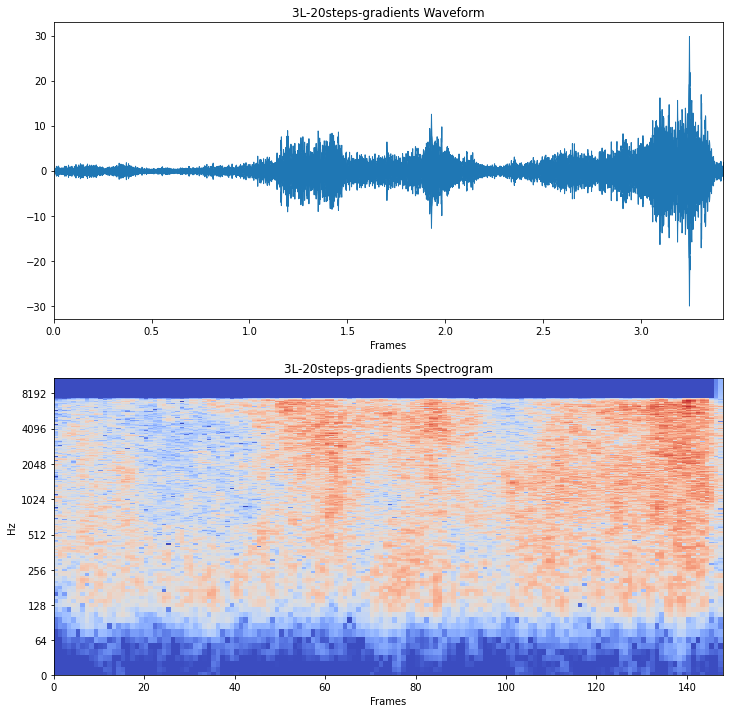
\includegraphics[width=0.5\textwidth]{dreamsound/3L-20steps-gradients.png}
       \caption{Taking last three layers, outputting gradients recursively for 20 steps.}
       \label{fig:img-6}
\end{figure*}
\begin{figure*}[htbp]
       \centering
              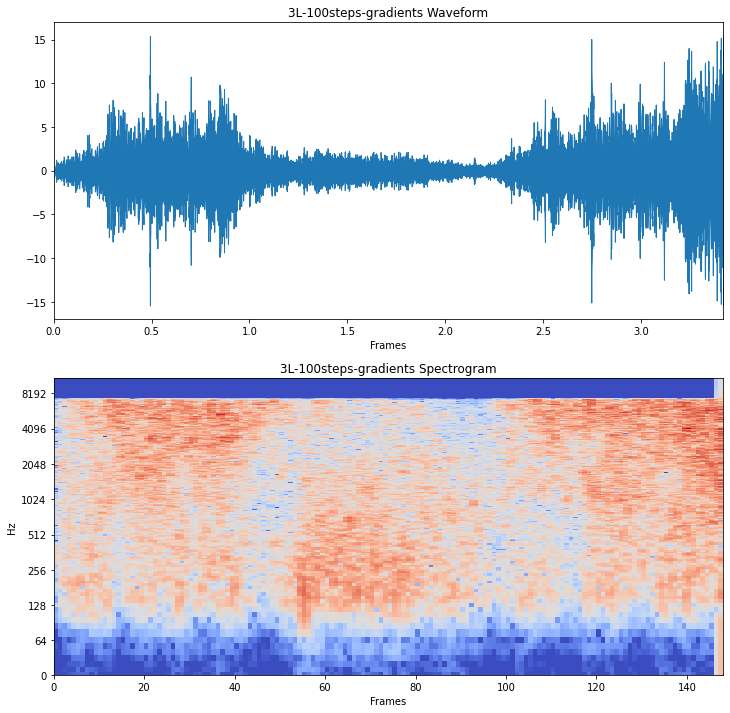
\includegraphics[width=0.5\textwidth]{dreamsound/L-100steps-gradients.png}
       \caption{Taking last 3 layers, for 100 steps, recursively feeding the gradients}
       \label{fig:img-7}
\end{figure*}
\section{Conclusions and Future Work}
We have presented a prototype adaptation of the Deep Dream project into an audio-based musical context using tensorflow and YAMNEt. We have contributed some research at the intersection of Deep Learning and audio-based musical tasks, and presented our results. The most interesting results occur when recursively applying an FFT filter built from the gradients obtained from an input soundfile and its loss. While our approach is tethered to a general sound database and a specific model, the techniques of gradient ascent for loss maximization of layer activations, and the FFT filter exposed in this paper are be portable enought for importing into other existing classification models for audio, such as for genre or musical instrument classification. Further, we plan on extending this project towards the creation of a database of dreamed sounds, with the capability to change models and other fft filtering techniques.

\section{Acknowledgments}
The authors would like to thank the reviewers, adding that the camera-ready paper will have a more detailed and verbose bibliographic section.
% \bibliographystyle{abbrv}
% \bibliography{dreamsound} 
\end{document}